\chapter{Design and Implementation}
\label{design}

%\section{Scenario}
%\section{Requeriments}
%\section{Design and Architecture}
%	\section{Related work}
%		\subsection{Using Pi-camera to stream}
%\section{Implementation}
%\section{Testing}
%\section{Software Quality}

\section{Introduction}
In this section, the design process that has been followed for the implementation of the application is going to be explained. First we find the requirements of the application, among which functional and non-functional requirements have been distinguished. Using these requirements, we explain how is the activity flow of the application. In this section are also included the prototypes and mockups that were used for designing the \gls{gui}. After, we can find an explanation of the architecture pattern followed along with the technologies that has been used in the project. In the next sections the interesting blocks of code of the front and back end are explained. 

%<+testing>

During the implementation of the system we found some issues that we had to face. In order to explain what these issues were and how they were overcome, the "Implementation Issues" section has been also included. Finally, at the end of this point we can find a summary of the implementation, with the lines of code (\glspl{loc}) of every file, and a little section about the quality of the software implemented. 

\section{Requirements}
From \cite{req_engineering_def}:

\say{The process to gather the software requirements from client, analyze and document them is known as \textit{requirement engineering}.}

In a real world project, the requirement engineering is a four step process: Feasibility Study, Requirement Gathering, Software Requirement Specification, Software Requirement Validation. However, in this project all roles are combined in one person, so the process is going to be more brief. We are going to assume that the first two steps are already done and directly going to create the Software Requirement Specification, where the following tables include the requirements that the system must follow.

	\subsection{Functional Requirements}
	The requirements have been divided in two different types. In this section we have included the functional requirements, which fall into "what the system should do".

	\begin{center}
		\begin{table}[h!b]
			\centering
		    \begin{tabular}{| c | c |}
			    \hline
			    ID & \makecell[c]{FR\textunderscore 01} \\ 
				\hline
				Priority & 
					\hspace{0.3cm} \checkedbox High \hspace{0.58cm} 
					\hspace{0.3cm} \uncheckedbox Medium \hspace{0.05cm}
					\hspace{0.3cm} \uncheckedbox Low \hspace{1.23cm} \\
			    \hline
			    Neccessity & 
					\hspace{0.3cm} \checkedbox Essential 
					\hspace{0.3cm} \uncheckedbox Desirable 
					\hspace{0.3cm} \uncheckedbox Optional \hspace{0.4cm} \\
			    \hline
			    Source & \makecell[c]{\checkedbox Client \hspace{1cm} \uncheckedbox Programmer \hspace{0.1cm}} \\ 
			    \hline
			    %						   -------------------------------------------------------|
			    Description & \makecell[c]{The system is divided in a client-server architecture.}    \\ 
			    \hline
			\end{tabular}
		    \caption{Functional Requirement FR\textunderscore 01}
		    \label{fr:01}
		\end{table}
		
		\begin{table}[h!b]
			\centering
		    \begin{tabular}{| c | c |}
			    \hline
			    ID & \makecell[c]{FR\textunderscore 02} \\ 
				\hline
				Priority & 
					\hspace{0.3cm} \checkedbox High \hspace{0.58cm} 
					\hspace{0.3cm} \uncheckedbox Medium \hspace{0.05cm}
					\hspace{0.3cm} \uncheckedbox Low \hspace{1.23cm} \\
			    \hline
			    Neccessity & 
					\hspace{0.3cm} \checkedbox Essential 
					\hspace{0.3cm} \uncheckedbox Desirable 
					\hspace{0.3cm} \uncheckedbox Optional \hspace{0.4cm} \\
			    \hline
			    Source & \makecell[c]{\checkedbox Client \hspace{1cm} \uncheckedbox Programmer \hspace{0.1cm}} \\ 
			    \hline
			    %						   -------------------------------------------------------|
			    Description & \makecell[c]{The Raspberry Pi will act as client of the server.}    \\ 
			    \hline
			\end{tabular}
		    \caption{Functional Requirement FR\textunderscore 02}
		    \label{fr:02}
		\end{table}
		
		\begin{table}[h!b]
			\centering
		    \begin{tabular}{| c | c |}
			    \hline
			    ID & \makecell[c]{FR\textunderscore 03} \\ 
				\hline
				Priority & 
					\hspace{0.3cm} \checkedbox High \hspace{0.58cm} 
					\hspace{0.3cm} \uncheckedbox Medium \hspace{0.05cm}
					\hspace{0.3cm} \uncheckedbox Low \hspace{1.23cm} \\
			    \hline
			    Neccessity & 
					\hspace{0.3cm} \checkedbox Essential 
					\hspace{0.3cm} \uncheckedbox Desirable 
					\hspace{0.3cm} \uncheckedbox Optional \hspace{0.4cm} \\
			    \hline
			    Source & \makecell[c]{\checkedbox Client \hspace{1cm} \uncheckedbox Programmer \hspace{0.1cm}} \\ 
			    \hline
			    %						   -------------------------------------------------------|
			    Description & \makecell[c]{The application will be executed in the Raspberry Pi.}    \\ 
			    \hline
			\end{tabular}
		    \caption{Functional Requirement FR\textunderscore 03}
		    \label{fr:03}
		\end{table}
		
		\begin{table}[h!b]
			\centering
		    \begin{tabular}{| c | c |}
			    \hline
			    ID & \makecell[c]{FR\textunderscore 04} \\ 
				\hline
				Priority & 
					\hspace{0.3cm} \checkedbox High \hspace{0.58cm} 
					\hspace{0.3cm} \uncheckedbox Medium \hspace{0.05cm}
					\hspace{0.3cm} \uncheckedbox Low \hspace{1.23cm} \\
			    \hline
			    Neccessity & 
					\hspace{0.3cm} \checkedbox Essential 
					\hspace{0.3cm} \uncheckedbox Desirable 
					\hspace{0.3cm} \uncheckedbox Optional \hspace{0.4cm} \\
			    \hline
			    Source & \makecell[c]{\checkedbox Client \hspace{1cm} \uncheckedbox Programmer \hspace{0.1cm}} \\ 
			    \hline
			    %						   -------------------------------------------------------|
			    Description & \makecell[c]{The application will have a \gls{gui}, so the users will\\ be able to interact with it.}    \\ 
			    \hline
			\end{tabular}
		    \caption{Functional Requirement FR\textunderscore 04}
		    \label{fr:04}
		\end{table}
		
		\begin{table}[h!b]
			\centering
		    \begin{tabular}{| c | c |}
			    \hline
			    ID & \makecell[c]{FR\textunderscore 05} \\ 
				\hline
				Priority & 
					\hspace{0.3cm} \uncheckedbox High \hspace{0.58cm} 
					\hspace{0.3cm} \checkedbox Medium \hspace{0.05cm}
					\hspace{0.3cm} \uncheckedbox Low \hspace{1.23cm} \\
			    \hline
			    Neccessity & 
					\hspace{0.3cm} \uncheckedbox Essential 
					\hspace{0.3cm} \uncheckedbox Desirable 
					\hspace{0.3cm} \checkedbox Optional \hspace{0.4cm} \\
			    \hline
			    Source & \makecell[c]{\checkedbox Client \hspace{1cm} \uncheckedbox Programmer \hspace{0.1cm}} \\ 
			    \hline
			    %						   -------------------------------------------------------|
			    Description & \makecell[c]{It will be able to close he applicationcan in any moment\\ pressing the Escape button.}    \\ 
			    \hline
			\end{tabular}
		    \caption{Functional Requirement FR\textunderscore 05}
		    \label{fr:05}
		\end{table}
		
		\begin{table}[h!b]
			\centering
		    \begin{tabular}{| c | c |}
			    \hline
			    ID & \makecell[c]{FR\textunderscore 06} \\ 
				\hline
				Priority & 
					\hspace{0.3cm} \checkedbox High \hspace{0.58cm} 
					\hspace{0.3cm} \uncheckedbox Medium \hspace{0.05cm}
					\hspace{0.3cm} \uncheckedbox Low \hspace{1.23cm} \\
			    \hline
			    Neccessity & 
					\hspace{0.3cm} \uncheckedbox Essential 
					\hspace{0.3cm} \checkedbox Desirable 
					\hspace{0.3cm} \uncheckedbox Optional \hspace{0.4cm} \\
			    \hline
			    Source & \makecell[c]{\checkedbox Client \hspace{1cm} \uncheckedbox Programmer \hspace{0.1cm}} \\ 
			    \hline
			    %						   -------------------------------------------------------|
			    Description & \makecell[c]{The application will show its status every time.}    \\ 
			    \hline
			\end{tabular}
		    \caption{Functional Requirement FR\textunderscore 06}
		    \label{fr:06}
		\end{table}
		
		\begin{table}[h!b]
			\centering
		    \begin{tabular}{| c | c |}
			    \hline
			    ID & \makecell[c]{FR\textunderscore 07} \\ 
				\hline
				Priority & 
					\hspace{0.3cm} \checkedbox High \hspace{0.58cm} 
					\hspace{0.3cm} \uncheckedbox Medium \hspace{0.05cm}
					\hspace{0.3cm} \uncheckedbox Low \hspace{1.23cm} \\
			    \hline
			    Neccessity & 
					\hspace{0.3cm} \checkedbox Essential 
					\hspace{0.3cm} \uncheckedbox Desirable 
					\hspace{0.3cm} \uncheckedbox Optional \hspace{0.4cm} \\
			    \hline
			    Source & \makecell[c]{\checkedbox Client \hspace{1cm} \uncheckedbox Programmer \hspace{0.1cm}} \\ 
			    \hline
			    %						   -------------------------------------------------------|
			    Description & \makecell[c]{The application will be divided in windows users can\\ navigate through.}    \\ 
			    \hline
			\end{tabular}
		    \caption{Functional Requirement FR\textunderscore 07}
		    \label{fr:07}
		\end{table}
		
		\begin{table}[h!b]
			\centering
		    \begin{tabular}{| c | c |}
			    \hline
			    ID & \makecell[c]{FR\textunderscore 08} \\ 
				\hline
				Priority & 
					\hspace{0.3cm} \uncheckedbox High \hspace{0.58cm} 
					\hspace{0.3cm} \checkedbox Medium \hspace{0.05cm}
					\hspace{0.3cm} \uncheckedbox Low \hspace{1.23cm} \\
			    \hline
			    Neccessity & 
					\hspace{0.3cm} \uncheckedbox Essential 
					\hspace{0.3cm} \checkedbox Desirable 
					\hspace{0.3cm} \uncheckedbox Optional \hspace{0.4cm} \\
			    \hline
			    Source & \makecell[c]{\checkedbox Client \hspace{1cm} \uncheckedbox Programmer \hspace{0.1cm}} \\ 
			    \hline
			    %						   -------------------------------------------------------|
			    Description & \makecell[c]{It will be possible to access the rest of windows.}    \\ 
			    \hline
			\end{tabular}
		    \caption{Functional Requirement FR\textunderscore 08}
		    \label{fr:08}
		\end{table}
		
		\begin{table}[h!b]
			\centering
		    \begin{tabular}{| c | c |}
			    \hline
			    ID & \makecell[c]{FR\textunderscore 09} \\ 
				\hline
				Priority & 
					\hspace{0.3cm} \checkedbox High \hspace{0.58cm} 
					\hspace{0.3cm} \uncheckedbox Medium \hspace{0.05cm}
					\hspace{0.3cm} \uncheckedbox Low \hspace{1.23cm} \\
			    \hline
			    Neccessity & 
					\hspace{0.3cm} \checkedbox Essential 
					\hspace{0.3cm} \uncheckedbox Desirable 
					\hspace{0.3cm} \uncheckedbox Optional \hspace{0.4cm} \\
			    \hline
			    Source & \makecell[c]{\uncheckedbox Client \hspace{1cm} \checkedbox Programmer \hspace{0.1cm}} \\ 
			    \hline
			    %						   -------------------------------------------------------|
			    Description & \makecell[c]{The access to the rest of the windows will be blocked\\ during the communication with the server.}    \\ 
			    \hline
			\end{tabular}
		    \caption{Functional Requirement FR\textunderscore 09}
		    \label{fr:09}
		\end{table}
		
		\begin{table}[h!b]
			\centering
		    \begin{tabular}{| c | c |}
			    \hline
			    ID & \makecell[c]{FR\textunderscore 10} \\ 
				\hline
				Priority & 
					\hspace{0.3cm} \checkedbox High \hspace{0.58cm} 
					\hspace{0.3cm} \uncheckedbox Medium \hspace{0.05cm}
					\hspace{0.3cm} \uncheckedbox Low \hspace{1.23cm} \\
			    \hline
			    Neccessity & 
					\hspace{0.3cm} \checkedbox Essential 
					\hspace{0.3cm} \uncheckedbox Desirable 
					\hspace{0.3cm} \uncheckedbox Optional \hspace{0.4cm} \\
			    \hline
			    Source & \makecell[c]{\checkedbox Client \hspace{1cm} \uncheckedbox Programmer \hspace{0.1cm}} \\ 
			    \hline
			    %						   -------------------------------------------------------|
			    Description & \makecell[c]{The face of the user will be recognised to identify\\
			    						    the user using a photo taken in the moment.}    \\ 
			    \hline
			\end{tabular}
		    \caption{Functional Requirement FR\textunderscore 10}
		    \label{fr:10}
		\end{table}
		
		\begin{table}[h!b]
			\centering
		    \begin{tabular}{| c | c |}
			    \hline
			    ID & \makecell[c]{FR\textunderscore 11} \\ 
				\hline
				Priority & 
					\hspace{0.3cm} \checkedbox High \hspace{0.58cm} 
					\hspace{0.3cm} \uncheckedbox Medium \hspace{0.05cm}
					\hspace{0.3cm} \uncheckedbox Low \hspace{1.23cm} \\
			    \hline
			    Neccessity & 
					\hspace{0.3cm} \checkedbox Essential 
					\hspace{0.3cm} \uncheckedbox Desirable 
					\hspace{0.3cm} \uncheckedbox Optional \hspace{0.4cm} \\
			    \hline
			    Source & \makecell[c]{\checkedbox Client \hspace{1cm} \uncheckedbox Programmer \hspace{0.1cm}} \\ 
			    \hline
			    %						   -------------------------------------------------------|
			    Description & \makecell[c]{A preview of the camera in real time will be shown\\ 
			    						   before the photo is taken.}    \\ 
			    \hline
			\end{tabular}
		    \caption{Functional Requirement FR\textunderscore 11}
		    \label{fr:11}
		\end{table}
		
		\begin{table}[h!b]
			\centering
		    \begin{tabular}{| c | c |}
			    \hline
			    ID & \makecell[c]{FR\textunderscore 12} \\ 
				\hline
				Priority & 
					\hspace{0.3cm} \uncheckedbox High \hspace{0.58cm} 
					\hspace{0.3cm} \checkedbox Medium \hspace{0.05cm}
					\hspace{0.3cm} \uncheckedbox Low \hspace{1.23cm} \\
			    \hline
			    Neccessity & 
					\hspace{0.3cm} \uncheckedbox Essential 
					\hspace{0.3cm} \checkedbox Desirable 
					\hspace{0.3cm} \uncheckedbox Optional \hspace{0.4cm} \\
			    \hline
			    Source & \makecell[c]{\checkedbox Client \hspace{1cm} \uncheckedbox Programmer \hspace{0.1cm}} \\ 
			    \hline
			    %						   -------------------------------------------------------|
			    Description & \makecell[c]{The user will be able to select the moment in which\\ 
			    						   the camera will take the photo.}    \\ 
			    \hline
			\end{tabular}
		    \caption{Functional Requirement FR\textunderscore 12}
		    \label{fr:12}
		\end{table}
		
		\begin{table}[h!b]
			\centering
		    \begin{tabular}{| c | c |}
			    \hline
			    ID & \makecell[c]{FR\textunderscore 13} \\ 
				\hline
				Priority & 
					\hspace{0.3cm} \uncheckedbox High \hspace{0.58cm} 
					\hspace{0.3cm} \checkedbox Medium \hspace{0.05cm}
					\hspace{0.3cm} \uncheckedbox Low \hspace{1.23cm} \\
			    \hline
			    Neccessity & 
					\hspace{0.3cm} \uncheckedbox Essential 
					\hspace{0.3cm} \checkedbox Desirable 
					\hspace{0.3cm} \uncheckedbox Optional \hspace{0.4cm} \\
			    \hline
			    Source & \makecell[c]{\checkedbox Client \hspace{1cm} \uncheckedbox Programmer \hspace{0.1cm}} \\ 
			    \hline
			    %						   -------------------------------------------------------|
			    Description & \makecell[c]{The user will be able to discard the taken photo and\\ 
			    						   take another one.}    \\ 
			    \hline
			\end{tabular}
		    \caption{Functional Requirement FR\textunderscore 13}
		    \label{fr:13}
		\end{table}
		
		\begin{table}[h!b]
			\centering
		    \begin{tabular}{| c | c |}
			    \hline
			    ID & \makecell[c]{FR\textunderscore 14} \\ 
				\hline
				Priority & 
					\hspace{0.3cm} \checkedbox High \hspace{0.58cm} 
					\hspace{0.3cm} \uncheckedbox Medium \hspace{0.05cm}
					\hspace{0.3cm} \uncheckedbox Low \hspace{1.23cm} \\
			    \hline
			    Neccessity & 
					\hspace{0.3cm} \checkedbox Essential 
					\hspace{0.3cm} \uncheckedbox Desirable 
					\hspace{0.3cm} \uncheckedbox Optional \hspace{0.4cm} \\
			    \hline
			    Source & \makecell[c]{\checkedbox Client \hspace{1cm} \uncheckedbox Programmer \hspace{0.1cm}} \\ 
			    \hline
			    %						   -------------------------------------------------------|
			    Description & \makecell[c]{The face recognition process will be able to recognise\\ 
			    						   only the students with which it has been trained.}    \\ 
			    \hline
			\end{tabular}
		    \caption{Functional Requirement FR\textunderscore 14}
		    \label{fr:14}
		\end{table}
		
		\begin{table}[h!b]
			\centering
		    \begin{tabular}{| c | c |}
			    \hline
			    ID & \makecell[c]{FR\textunderscore 15} \\ 
				\hline
				Priority & 
					\hspace{0.3cm} \checkedbox High \hspace{0.58cm} 
					\hspace{0.3cm} \uncheckedbox Medium \hspace{0.05cm}
					\hspace{0.3cm} \uncheckedbox Low \hspace{1.23cm} \\
			    \hline
			    Neccessity & 
					\hspace{0.3cm} \checkedbox Essential 
					\hspace{0.3cm} \uncheckedbox Desirable 
					\hspace{0.3cm} \uncheckedbox Optional \hspace{0.4cm} \\
			    \hline
			    Source & \makecell[c]{\checkedbox Client \hspace{1cm} \uncheckedbox Programmer \hspace{0.1cm}} \\ 
			    \hline
			    %						   -------------------------------------------------------|
			    Description & \makecell[c]{The server will have a route in order to perform the \\
			    						   face recognition in which an image will be required\\ 
			    						   as a parameter.}    \\ 
			    \hline
			\end{tabular}
		    \caption{Functional Requirement FR\textunderscore 15}
		    \label{fr:15}
		\end{table}
		
		\begin{table}[h!b]
			\centering
		    \begin{tabular}{| c | c |}
			    \hline
			    ID & \makecell[c]{FR\textunderscore 16} \\ 
				\hline
				Priority & 
					\hspace{0.3cm} \checkedbox High \hspace{0.58cm} 
					\hspace{0.3cm} \uncheckedbox Medium \hspace{0.05cm}
					\hspace{0.3cm} \uncheckedbox Low \hspace{1.23cm} \\
			    \hline
			    Neccessity & 
					\hspace{0.3cm} \uncheckedbox Essential 
					\hspace{0.3cm} \checkedbox Desirable 
					\hspace{0.3cm} \uncheckedbox Optional \hspace{0.4cm} \\
			    \hline
			    Source & \makecell[c]{\checkedbox Client \hspace{1cm} \uncheckedbox Programmer \hspace{0.1cm}} \\ 
			    \hline
			    %						   -------------------------------------------------------|
			    Description & \makecell[c]{The application will show a loading screen during the\\ 
			    						   communication with the server.}    \\ 
			    \hline
			\end{tabular}
		    \caption{Functional Requirement FR\textunderscore 16}
		    \label{fr:16}
		\end{table}
		
		\begin{table}[h!b]
			\centering
		    \begin{tabular}{| c | c |}
			    \hline
			    ID & \makecell[c]{FR\textunderscore 17} \\ 
				\hline
				Priority & 
					\hspace{0.3cm} \checkedbox High \hspace{0.58cm} 
					\hspace{0.3cm} \uncheckedbox Medium \hspace{0.05cm}
					\hspace{0.3cm} \uncheckedbox Low \hspace{1.23cm} \\
			    \hline
			    Neccessity & 
					\hspace{0.3cm} \checkedbox Essential 
					\hspace{0.3cm} \uncheckedbox Desirable 
					\hspace{0.3cm} \uncheckedbox Optional \hspace{0.4cm} \\
			    \hline
			    Source & \makecell[c]{\checkedbox Client \hspace{1cm} \uncheckedbox Programmer \hspace{0.1cm}} \\ 
			    \hline
			    %						   -------------------------------------------------------|
			    Description & \makecell[c]{The student's photo will be stored in the server during\\
			    						   the time the request is being processed. }    \\ 
			    \hline
			\end{tabular}
		    \caption{Functional Requirement FR\textunderscore 17}
		    \label{fr:17}
		\end{table}
		
		\begin{table}[h!b]
			\centering
		    \begin{tabular}{| c | c |}
			    \hline
			    ID & \makecell[c]{FR\textunderscore 18} \\ 
				\hline
				Priority & 
					\hspace{0.3cm} \checkedbox High \hspace{0.58cm} 
					\hspace{0.3cm} \uncheckedbox Medium \hspace{0.05cm}
					\hspace{0.3cm} \uncheckedbox Low \hspace{1.23cm} \\
			    \hline
			    Neccessity & 
					\hspace{0.3cm} \checkedbox Essential 
					\hspace{0.3cm} \uncheckedbox Desirable 
					\hspace{0.3cm} \uncheckedbox Optional \hspace{0.4cm} \\
			    \hline
			    Source & \makecell[c]{\checkedbox Client \hspace{1cm} \uncheckedbox Programmer \hspace{0.1cm}} \\ 
			    \hline
			    %						   -------------------------------------------------------|
			    Description & \makecell[c]{The student's photo will be deleted after the face\\
			    						   recognition process.}    \\ 
			    \hline
			\end{tabular}
		    \caption{Functional Requirement FR\textunderscore 18}
		    \label{fr:18}
		\end{table}
		
		\begin{table}[h!b]
			\centering
		    \begin{tabular}{| c | c |}
			    \hline
			    ID & \makecell[c]{FR\textunderscore 19} \\ 
				\hline
				Priority & 
					\hspace{0.3cm} \checkedbox High \hspace{0.58cm} 
					\hspace{0.3cm} \uncheckedbox Medium \hspace{0.05cm}
					\hspace{0.3cm} \uncheckedbox Low \hspace{1.23cm} \\
			    \hline
			    Neccessity & 
					\hspace{0.3cm} \checkedbox Essential 
					\hspace{0.3cm} \uncheckedbox Desirable 
					\hspace{0.3cm} \uncheckedbox Optional \hspace{0.4cm} \\
			    \hline
			    Source & \makecell[c]{\checkedbox Client \hspace{1cm} \uncheckedbox Programmer \hspace{0.1cm}} \\ 
			    \hline
			    %						   -------------------------------------------------------|
			    Description & \makecell[c]{The student's photo will be pre-processed applying face\\
			    						   detection and cropping the face of the student.}    \\ 
			    \hline
			\end{tabular}
		    \caption{Functional Requirement FR\textunderscore 19}
		    \label{fr:19}
		\end{table}
		
		\begin{table}[h!b]
			\centering
		    \begin{tabular}{| c | c |}
			    \hline
			    ID & \makecell[c]{FR\textunderscore 20} \\ 
				\hline
				Priority & 
					\hspace{0.3cm} \checkedbox High \hspace{0.58cm} 
					\hspace{0.3cm} \uncheckedbox Medium \hspace{0.05cm}
					\hspace{0.3cm} \uncheckedbox Low \hspace{1.23cm} \\
			    \hline
			    Neccessity & 
					\hspace{0.3cm} \checkedbox Essential 
					\hspace{0.3cm} \uncheckedbox Desirable 
					\hspace{0.3cm} \uncheckedbox Optional \hspace{0.4cm} \\
			    \hline
			    Source & \makecell[c]{\checkedbox Client \hspace{1cm} \uncheckedbox Programmer \hspace{0.1cm}} \\ 
			    \hline
			    %						   -------------------------------------------------------|
			    Description & \makecell[c]{The application will show a window with a message reporting\\
			    						   the failed face detection process, if necessary.}    \\ 
			    \hline
			\end{tabular}
		    \caption{Functional Requirement FR\textunderscore 20}
		    \label{fr:20}
		\end{table}
		
		\begin{table}[h!b]
			\centering
		    \begin{tabular}{| c | c |}
			    \hline
			    ID & \makecell[c]{FR\textunderscore 21} \\ 
				\hline
				Priority & 
					\hspace{0.3cm} \checkedbox High \hspace{0.58cm} 
					\hspace{0.3cm} \uncheckedbox Medium \hspace{0.05cm}
					\hspace{0.3cm} \uncheckedbox Low \hspace{1.23cm} \\
			    \hline
			    Neccessity & 
					\hspace{0.3cm} \checkedbox Essential 
					\hspace{0.3cm} \uncheckedbox Desirable 
					\hspace{0.3cm} \uncheckedbox Optional \hspace{0.4cm} \\
			    \hline
			    Source & \makecell[c]{\checkedbox Client \hspace{1cm} \uncheckedbox Programmer \hspace{0.1cm}} \\ 
			    \hline
			    %						   -------------------------------------------------------|
			    Description & \makecell[c]{The face recognition process will be done using the \\
			    						   pre-processed photo.}    \\ 
			    \hline
			\end{tabular}
		    \caption{Functional Requirement FR\textunderscore 21}
		    \label{fr:21}
		\end{table}
		
		\begin{table}[h!b]
			\centering
		    \begin{tabular}{| c | c |}
			    \hline
			    ID & \makecell[c]{FR\textunderscore 22} \\ 
				\hline
				Priority & 
					\hspace{0.3cm} \checkedbox High \hspace{0.58cm} 
					\hspace{0.3cm} \uncheckedbox Medium \hspace{0.05cm}
					\hspace{0.3cm} \uncheckedbox Low \hspace{1.23cm} \\
			    \hline
			    Neccessity & 
					\hspace{0.3cm} \checkedbox Essential 
					\hspace{0.3cm} \uncheckedbox Desirable 
					\hspace{0.3cm} \uncheckedbox Optional \hspace{0.4cm} \\
			    \hline
			    Source & \makecell[c]{\checkedbox Client \hspace{1cm} \uncheckedbox Programmer \hspace{0.1cm}} \\ 
			    \hline
			    %						   -------------------------------------------------------|
			    Description & \makecell[c]{The application will show a window with a message reporting\\ 
			    						   the failed face recognition process, if necessary.}    \\ 
			    \hline
			\end{tabular}
		    \caption{Functional Requirement FR\textunderscore 22}
		    \label{fr:22}
		\end{table}
		
		\begin{table}[h!b]
			\centering
		    \begin{tabular}{| c | c |}
			    \hline
			    ID & \makecell[c]{FR\textunderscore 23} \\ 
				\hline
				Priority & 
					\hspace{0.3cm} \checkedbox High \hspace{0.58cm} 
					\hspace{0.3cm} \uncheckedbox Medium \hspace{0.05cm}
					\hspace{0.3cm} \uncheckedbox Low \hspace{1.23cm} \\
			    \hline
			    Neccessity & 
					\hspace{0.3cm} \checkedbox Essential 
					\hspace{0.3cm} \uncheckedbox Desirable 
					\hspace{0.3cm} \uncheckedbox Optional \hspace{0.4cm} \\
			    \hline
			    Source & \makecell[c]{\checkedbox Client \hspace{1cm} \uncheckedbox Programmer \hspace{0.1cm}} \\ 
			    \hline
			    %						   -------------------------------------------------------|
			    Description & \makecell[c]{The server will have a database that is loaded with\\
			    						   the name of the students and their associated ID number. }    \\ 
			    \hline
			\end{tabular}
		    \caption{Functional Requirement FR\textunderscore 23}
		    \label{fr:23}
		\end{table}
		
		\begin{table}[h!b]
			\centering
		    \begin{tabular}{| c | c |}
			    \hline
			    ID & \makecell[c]{FR\textunderscore 24} \\ 
				\hline
				Priority & 
					\hspace{0.3cm} \checkedbox High \hspace{0.58cm} 
					\hspace{0.3cm} \uncheckedbox Medium \hspace{0.05cm}
					\hspace{0.3cm} \uncheckedbox Low \hspace{1.23cm} \\
			    \hline
			    Neccessity & 
					\hspace{0.3cm} \checkedbox Essential 
					\hspace{0.3cm} \uncheckedbox Desirable 
					\hspace{0.3cm} \uncheckedbox Optional \hspace{0.4cm} \\
			    \hline
			    Source & \makecell[c]{\checkedbox Client \hspace{1cm} \uncheckedbox Programmer \hspace{0.1cm}} \\ 
			    \hline
			    %						   -------------------------------------------------------|
			    Description & \makecell[c]{After the face recognition process, the server will\\
			    						   send back the name of the student and their associated\\
			    						   ID number.}    \\ 
			    \hline
			\end{tabular}
		    \caption{Functional Requirement FR\textunderscore 24}
		    \label{fr:24}
		\end{table}
		
		\begin{table}[h!b]
			\centering
		    \begin{tabular}{| c | c |}
			    \hline
			    ID & \makecell[c]{FR\textunderscore 25} \\ 
				\hline
				Priority & 
					\hspace{0.3cm} \uncheckedbox High \hspace{0.58cm} 
					\hspace{0.3cm} \uncheckedbox Medium \hspace{0.05cm}
					\hspace{0.3cm} \checkedbox Low \hspace{1.23cm} \\
			    \hline
			    Neccessity & 
					\hspace{0.3cm} \uncheckedbox Essential 
					\hspace{0.3cm} \uncheckedbox Desirable 
					\hspace{0.3cm} \checkedbox Optional \hspace{0.4cm} \\
			    \hline
			    Source & \makecell[c]{\checkedbox Client \hspace{1cm} \uncheckedbox Programmer \hspace{0.1cm}} \\ 
			    \hline
			    %						   -------------------------------------------------------|
			    Description & \makecell[c]{The application will show a window with a message \\
			    						   welcoming the student using their name.}    \\ 
			    \hline
			\end{tabular}
		    \caption{Functional Requirement FR\textunderscore 25}
		    \label{fr:25}
		\end{table}
		
		\begin{table}[h!b]
			\centering
		    \begin{tabular}{| c | c |}
			    \hline
			    ID & \makecell[c]{FR\textunderscore 26} \\ 
				\hline
				Priority & 
					\hspace{0.3cm} \checkedbox High \hspace{0.58cm} 
					\hspace{0.3cm} \uncheckedbox Medium \hspace{0.05cm}
					\hspace{0.3cm} \uncheckedbox Low \hspace{1.23cm} \\
			    \hline
			    Neccessity & 
					\hspace{0.3cm} \checkedbox Essential 
					\hspace{0.3cm} \uncheckedbox Desirable 
					\hspace{0.3cm} \uncheckedbox Optional \hspace{0.4cm} \\
			    \hline
			    Source & \makecell[c]{\checkedbox Client \hspace{1cm} \uncheckedbox Programmer \hspace{0.1cm}} \\ 
			    \hline
			    %						   -------------------------------------------------------|
			    Description & \makecell[c]{The server will have a route in order to get the next\\
			    						   class of the student in which a student's ID number\\
			    						   will be required as a parameter.}    \\ 
			    \hline
			\end{tabular}
		    \caption{Functional Requirement FR\textunderscore 26}
		    \label{fr:26}
		\end{table}
		
		\begin{table}[h!b]
			\centering
		    \begin{tabular}{| c | c |}
			    \hline
			    ID & \makecell[c]{FR\textunderscore 27} \\ 
				\hline
				Priority & 
					\hspace{0.3cm} \checkedbox High \hspace{0.58cm} 
					\hspace{0.3cm} \uncheckedbox Medium \hspace{0.05cm}
					\hspace{0.3cm} \uncheckedbox Low \hspace{1.23cm} \\
			    \hline
			    Neccessity & 
					\hspace{0.3cm} \checkedbox Essential 
					\hspace{0.3cm} \uncheckedbox Desirable 
					\hspace{0.3cm} \uncheckedbox Optional \hspace{0.4cm} \\
			    \hline
			    Source & \makecell[c]{\checkedbox Client \hspace{1cm} \uncheckedbox Programmer \hspace{0.1cm}} \\ 
			    \hline
			    %						   -------------------------------------------------------|
			    Description & \makecell[c]{The server will gls{scrape} the timetable.ul.ie \\
			    						   website to obtain the timetable of the student.}    \\ 
			    \hline
			\end{tabular}
		    \caption{Functional Requirement FR\textunderscore 27}
		    \label{fr:27}
		\end{table}
		
		\begin{table}[h!b]
			\centering
		    \begin{tabular}{| c | c |}
			    \hline
			    ID & \makecell[c]{FR\textunderscore 28} \\ 
				\hline
				Priority & 
					\hspace{0.3cm} \checkedbox High \hspace{0.58cm} 
					\hspace{0.3cm} \uncheckedbox Medium \hspace{0.05cm}
					\hspace{0.3cm} \uncheckedbox Low \hspace{1.23cm} \\
			    \hline
			    Neccessity & 
					\hspace{0.3cm} \uncheckedbox Essential 
					\hspace{0.3cm} \checkedbox Desirable 
					\hspace{0.3cm} \uncheckedbox Optional \hspace{0.4cm} \\
			    \hline
			    Source & \makecell[c]{\checkedbox Client \hspace{1cm} \uncheckedbox Programmer \hspace{0.1cm}} \\ 
			    \hline
			    %						   -------------------------------------------------------|
			    Description & \makecell[c]{The server will analise the data obtained from the \\
			    						   website to obtain the next class of the student.}    \\ 
			    \hline
			\end{tabular}
		    \caption{Functional Requirement FR\textunderscore 28}
		    \label{fr:28}
		\end{table}
		
		\begin{table}[h!b]
			\centering
		    \begin{tabular}{| c | c |}
			    \hline
			    ID & \makecell[c]{FR\textunderscore 29} \\ 
				\hline
				Priority & 
					\hspace{0.3cm} \checkedbox High \hspace{0.58cm} 
					\hspace{0.3cm} \uncheckedbox Medium \hspace{0.05cm}
					\hspace{0.3cm} \uncheckedbox Low \hspace{1.23cm} \\
			    \hline
			    Neccessity & 
					\hspace{0.3cm} \checkedbox Essential 
					\hspace{0.3cm} \uncheckedbox Desirable 
					\hspace{0.3cm} \uncheckedbox Optional \hspace{0.4cm} \\
			    \hline
			    Source & \makecell[c]{\checkedbox Client \hspace{1cm} \uncheckedbox Programmer \hspace{0.1cm}} \\ 
			    \hline
			    %						   -------------------------------------------------------|
			    Description & \makecell[c]{After the next class of the student is obtained, the \\
			    						   server will send back the data of the next class, which \\
			    						   include: code of the module, name of the module, \\
			    						   starting hour, ending hour, class type and location.}    \\ 
			    \hline
			\end{tabular}
		    \caption{Functional Requirement FR\textunderscore 29}
		    \label{fr:29}
		\end{table}
		
		\begin{table}[h!b]
			\centering
		    \begin{tabular}{| c | c |}
			    \hline
			    ID & \makecell[c]{FR\textunderscore 30} \\ 
				\hline
				Priority & 
					\hspace{0.3cm} \checkedbox High \hspace{0.58cm} 
					\hspace{0.3cm} \uncheckedbox Medium \hspace{0.05cm}
					\hspace{0.3cm} \uncheckedbox Low \hspace{1.23cm} \\
			    \hline
			    Neccessity & 
					\hspace{0.3cm} \checkedbox Essential 
					\hspace{0.3cm} \uncheckedbox Desirable 
					\hspace{0.3cm} \uncheckedbox Optional \hspace{0.4cm} \\
			    \hline
			    Source & \makecell[c]{\checkedbox Client \hspace{1cm} \uncheckedbox Programmer \hspace{0.1cm}} \\ 
			    \hline
			    %						   -------------------------------------------------------|
			    Description & \makecell[c]{The application will show a window with a message \\
			    						   reporting that the user has no more classes in that \\
			    						   day, if necessary.}    \\ 
			    \hline
			\end{tabular}
		    \caption{Functional Requirement FR\textunderscore 30}
		    \label{fr:30}
		\end{table}
		
		\begin{table}[h!b]
			\centering
		    \begin{tabular}{| c | c |}
			    \hline
			    ID & \makecell[c]{FR\textunderscore 31} \\ 
				\hline
				Priority & 
					\hspace{0.3cm} \checkedbox High \hspace{0.58cm} 
					\hspace{0.3cm} \uncheckedbox Medium \hspace{0.05cm}
					\hspace{0.3cm} \uncheckedbox Low \hspace{1.23cm} \\
			    \hline
			    Neccessity & 
					\hspace{0.3cm} \checkedbox Essential 
					\hspace{0.3cm} \uncheckedbox Desirable 
					\hspace{0.3cm} \uncheckedbox Optional \hspace{0.4cm} \\
			    \hline
			    Source & \makecell[c]{\checkedbox Client \hspace{1cm} \uncheckedbox Programmer \hspace{0.1cm}} \\ 
			    \hline
			    %						   -------------------------------------------------------|
			    Description & \makecell[c]{The application will show a window with the data of \\
			    						   the next class of the student.}    \\ 
			    \hline
			\end{tabular}
		    \caption{Functional Requirement FR\textunderscore 31}
		    \label{fr:31}
		\end{table}
		
		\begin{table}[h!b]
			\centering
		    \begin{tabular}{| c | c |}
			    \hline
			    ID & \makecell[c]{FR\textunderscore 32} \\ 
				\hline
				Priority & 
					\hspace{0.3cm} \checkedbox High \hspace{0.58cm} 
					\hspace{0.3cm} \uncheckedbox Medium \hspace{0.05cm}
					\hspace{0.3cm} \uncheckedbox Low \hspace{1.23cm} \\
			    \hline
			    Neccessity & 
					\hspace{0.3cm} \checkedbox Essential 
					\hspace{0.3cm} \uncheckedbox Desirable 
					\hspace{0.3cm} \uncheckedbox Optional \hspace{0.4cm} \\
			    \hline
			    Source & \makecell[c]{\checkedbox Client \hspace{1cm} \uncheckedbox Programmer \hspace{0.1cm}} \\ 
			    \hline
			    %						   -------------------------------------------------------|
			    Description & \makecell[c]{The server will have a route in order to get map to \\
			    						   the next class of the student in which the origin and \\
			    						   destination locations will be required as parameters.}    \\ 
			    \hline
			\end{tabular}
		    \caption{Functional Requirement FR\textunderscore 32}
		    \label{fr:32}
		\end{table}
		
		\begin{table}[h!b]
			\centering
		    \begin{tabular}{| c | c |}
			    \hline
			    ID & \makecell[c]{FR\textunderscore 33} \\ 
				\hline
				Priority & 
					\hspace{0.3cm} \checkedbox High \hspace{0.58cm} 
					\hspace{0.3cm} \uncheckedbox Medium \hspace{0.05cm}
					\hspace{0.3cm} \uncheckedbox Low \hspace{1.23cm} \\
			    \hline
			    Neccessity & 
					\hspace{0.3cm} \checkedbox Essential 
					\hspace{0.3cm} \uncheckedbox Desirable 
					\hspace{0.3cm} \uncheckedbox Optional \hspace{0.4cm} \\
			    \hline
			    Source & \makecell[c]{\checkedbox Client \hspace{1cm} \uncheckedbox Programmer \hspace{0.1cm}} \\ 
			    \hline
			    %						   -------------------------------------------------------|
			    Description & \makecell[c]{The map to the next class of the student will show the\\
			    						    origin point, the destination point and the path from\\
			    						    one to another.}    \\ 
			    \hline
			\end{tabular}
		    \caption{Functional Requirement FR\textunderscore 33}
		    \label{fr:33}
		\end{table}
		
		\begin{table}[h!b]
			\centering
		    \begin{tabular}{| c | c |}
			    \hline
			    ID & \makecell[c]{FR\textunderscore 34} \\ 
				\hline
				Priority & 
					\hspace{0.3cm} \uncheckedbox High \hspace{0.58cm} 
					\hspace{0.3cm} \checkedbox Medium \hspace{0.05cm}
					\hspace{0.3cm} \uncheckedbox Low \hspace{1.23cm} \\
			    \hline
			    Neccessity & 
					\hspace{0.3cm} \uncheckedbox Essential 
					\hspace{0.3cm} \checkedbox Desirable 
					\hspace{0.3cm} \uncheckedbox Optional \hspace{0.4cm} \\
			    \hline
			    Source & \makecell[c]{\uncheckedbox Client \hspace{1cm} \checkedbox Programmer \hspace{0.1cm}} \\ 
			    \hline
			    %						   -------------------------------------------------------|
			    Description & \makecell[c]{The server will obtain the map as an image.}    \\ 
			    \hline
			\end{tabular}
		    \caption{Functional Requirement FR\textunderscore 34}
		    \label{fr:34}
		\end{table}
		
		\begin{table}[h!b]
			\centering
		    \begin{tabular}{| c | c |}
			    \hline
			    ID & \makecell[c]{FR\textunderscore 35} \\ 
				\hline
				Priority & 
					\hspace{0.3cm} \checkedbox High \hspace{0.58cm} 
					\hspace{0.3cm} \uncheckedbox Medium \hspace{0.05cm}
					\hspace{0.3cm} \uncheckedbox Low \hspace{1.23cm} \\
			    \hline
			    Neccessity & 
					\hspace{0.3cm} \checkedbox Essential 
					\hspace{0.3cm} \uncheckedbox Desirable 
					\hspace{0.3cm} \uncheckedbox Optional \hspace{0.4cm} \\
			    \hline
			    Source & \makecell[c]{\uncheckedbox Client \hspace{1cm} \checkedbox Programmer \hspace{0.1cm}} \\ 
			    \hline
			    %						   -------------------------------------------------------|
			    Description & \makecell[c]{The server will send back the map as an image.}    \\ 
			    \hline
			\end{tabular}
		    \caption{Functional Requirement FR\textunderscore 35}
		    \label{fr:35}
		\end{table}
		
		\begin{table}[h!b]
			\centering
		    \begin{tabular}{| c | c |}
			    \hline
			    ID & \makecell[c]{FR\textunderscore 36} \\ 
				\hline
				Priority & 
					\hspace{0.3cm} \checkedbox High \hspace{0.58cm} 
					\hspace{0.3cm} \uncheckedbox Medium \hspace{0.05cm}
					\hspace{0.3cm} \uncheckedbox Low \hspace{1.23cm} \\
			    \hline
			    Neccessity & 
					\hspace{0.3cm} \checkedbox Essential 
					\hspace{0.3cm} \uncheckedbox Desirable 
					\hspace{0.3cm} \uncheckedbox Optional \hspace{0.4cm} \\
			    \hline
			    Source & \makecell[c]{\checkedbox Client \hspace{1cm} \uncheckedbox Programmer \hspace{0.1cm}} \\ 
			    \hline
			    %						   -------------------------------------------------------|
			    Description & \makecell[c]{The application will show a window with the map from \\
			    						   the current location of the student to their next class.}    \\ 
			    \hline
			\end{tabular}
		    \caption{Functional Requirement FR\textunderscore 36}
		    \label{fr:36}
		\end{table}
		
		\begin{table}[h!b]
			\centering
		    \begin{tabular}{| c | c |}
			    \hline
			    ID & \makecell[c]{FR\textunderscore 37} \\ 
				\hline
				Priority & 
					\hspace{0.3cm} \uncheckedbox High \hspace{0.58cm} 
					\hspace{0.3cm} \checkedbox Medium \hspace{0.05cm}
					\hspace{0.3cm} \uncheckedbox Low \hspace{1.23cm} \\
			    \hline
			    Neccessity & 
					\hspace{0.3cm} \uncheckedbox Essential 
					\hspace{0.3cm} \checkedbox Desirable 
					\hspace{0.3cm} \uncheckedbox Optional \hspace{0.4cm} \\
			    \hline
			    Source & \makecell[c]{\checkedbox Client \hspace{1cm} \uncheckedbox Programmer \hspace{0.1cm}} \\ 
			    \hline
			    %						   -------------------------------------------------------|
			    Description & \makecell[c]{The windows that show the data of the next class of \\
			    						   the student and the map, will be not accessible when \\
			    						   the application stars.}    \\ 
			    \hline
			\end{tabular}
		    \caption{Functional Requirement FR\textunderscore 37}
		    \label{fr:37}
		\end{table}
		
		\begin{table}[h!b]
			\centering
		    \begin{tabular}{| c | c |}
			    \hline
			    ID & \makecell[c]{FR\textunderscore 38} \\ 
				\hline
				Priority & 
					\hspace{0.3cm} \uncheckedbox High \hspace{0.58cm} 
					\hspace{0.3cm} \checkedbox Medium \hspace{0.05cm}
					\hspace{0.3cm} \uncheckedbox Low \hspace{1.23cm} \\
			    \hline
			    Neccessity & 
					\hspace{0.3cm} \uncheckedbox Essential 
					\hspace{0.3cm} \checkedbox Desirable 
					\hspace{0.3cm} \uncheckedbox Optional \hspace{0.4cm} \\
			    \hline
			    Source & \makecell[c]{\checkedbox Client \hspace{1cm} \uncheckedbox Programmer \hspace{0.1cm}} \\ 
			    \hline
			    %						   -------------------------------------------------------|
			    Description & \makecell[c]{The windows that show the data of the next class of \\
			    						   the student and the map, will be not accessible when \\
			    						   the application does not detect or recognise the \\
			    						   user's face.}    \\ 
			    \hline
			\end{tabular}
		    \caption{Functional Requirement FR\textunderscore 38}
		    \label{fr:38}
		\end{table}

		\begin{table}[h!b]
			\centering
		    \begin{tabular}{| c | c |}
			    \hline
			    ID & \makecell[c]{FR\textunderscore 39} \\ 
				\hline
				Priority & 
					\hspace{0.3cm} \checkedbox High \hspace{0.58cm} 
					\hspace{0.3cm} \uncheckedbox Medium \hspace{0.05cm}
					\hspace{0.3cm} \uncheckedbox Low \hspace{1.23cm} \\
			    \hline
			    Neccessity & 
					\hspace{0.3cm} \uncheckedbox Essential 
					\hspace{0.3cm} \checkedbox Desirable 
					\hspace{0.3cm} \uncheckedbox Optional \hspace{0.4cm} \\
			    \hline
			    Source & \makecell[c]{\checkedbox Client \hspace{1cm} \uncheckedbox Programmer \hspace{0.1cm}} \\ 
			    \hline
			    %						   -------------------------------------------------------|
			    Description & \makecell[c]{The windows that show the data of the next class of \\
			    						   the student and the map, will be accessible in the \\
			    						   moment the student is recognised and that student has a\\
			    						   class after in the day.}    \\ 
			    \hline
			\end{tabular}
		    \caption{Functional Requirement FR\textunderscore 39}
		    \label{fr:39}
		\end{table}

	\end{center}

	\clearpage


	\subsection{Non-functional Requirements}
	The requirements have been divided in two different types. In this section we have included the non-functional requirements, which fall into "how the system performs a certain function".

	\begin{center}

		\begin{table}[h!b]
			\centering
		    \begin{tabular}{| c | c |}
			    \hline
			    ID & \makecell[c]{NFR\textunderscore 01} \\ 
				\hline
				Priority & 
					\hspace{0.3cm} \checkedbox High \hspace{0.58cm} 
					\hspace{0.3cm} \uncheckedbox Medium \hspace{0.05cm}
					\hspace{0.3cm} \uncheckedbox Low \hspace{1.23cm} \\
			    \hline
			    Neccessity & 
					\hspace{0.3cm} \checkedbox Essential 
					\hspace{0.3cm} \uncheckedbox Desirable 
					\hspace{0.3cm} \uncheckedbox Optional \hspace{0.4cm} \\
			    \hline
			    Source & \makecell[c]{\checkedbox Client \hspace{1cm} \uncheckedbox Programmer \hspace{0.1cm}} \\ 
			    \hline
			    %						   -------------------------------------------------------|
			    Description & \makecell[c]{Client and server will interact with each other using \\
			    						   the HTTP protocol.}    \\ 
			    \hline
			\end{tabular}
		    \caption{Non\textendash Functional Requirement NFR\textunderscore 01}
		    \label{nfr:01}
		\end{table}

		\begin{table}[h!b]
			\centering
		    \begin{tabular}{| c | c |}
			    \hline
			    ID & \makecell[c]{NFR\textunderscore 02} \\ 
				\hline
				Priority & 
					\hspace{0.3cm} \checkedbox High \hspace{0.58cm} 
					\hspace{0.3cm} \uncheckedbox Medium \hspace{0.05cm}
					\hspace{0.3cm} \uncheckedbox Low \hspace{1.23cm} \\
			    \hline
			    Neccessity & 
					\hspace{0.3cm} \checkedbox Essential 
					\hspace{0.3cm} \uncheckedbox Desirable 
					\hspace{0.3cm} \uncheckedbox Optional \hspace{0.4cm} \\
			    \hline
			    Source & \makecell[c]{\checkedbox Client \hspace{1cm} \uncheckedbox Programmer \hspace{0.1cm}} \\ 
			    \hline
			    %						   -------------------------------------------------------|
			    Description & \makecell[c]{The data in the HTTP requests and responses will be \\
			    						   formatted using JSON.}    \\ 
			    \hline
			\end{tabular}
		    \caption{Non\textendash Functional Requirement NFR\textunderscore 02}
		    \label{nfr:02}
		\end{table}
		
		\begin{table}[h!b]
			\centering
		    \begin{tabular}{| c | c |}
			    \hline
			    ID & \makecell[c]{NFR\textunderscore 03} \\ 
				\hline
				Priority & 
					\hspace{0.3cm} \checkedbox High \hspace{0.58cm} 
					\hspace{0.3cm} \uncheckedbox Medium \hspace{0.05cm}
					\hspace{0.3cm} \uncheckedbox Low \hspace{1.23cm} \\
			    \hline
			    Neccessity & 
					\hspace{0.3cm} \uncheckedbox Essential 
					\hspace{0.3cm} \checkedbox Desirable 
					\hspace{0.3cm} \uncheckedbox Optional \hspace{0.4cm} \\
			    \hline
			    Source & \makecell[c]{\uncheckedbox Client \hspace{1cm} \checkedbox Programmer \hspace{0.1cm}} \\ 
			    \hline
			    %						   -------------------------------------------------------|
			    Description & \makecell[c]{Client and server will be located in the same network.}    \\ 
			    \hline
			\end{tabular}
		    \caption{Non\textendash Functional Requirement NFR\textunderscore 03}
		    \label{nfr:03}
		\end{table}
		
		\begin{table}[h!b]
			\centering
		    \begin{tabular}{| c | c |}
			    \hline
			    ID & \makecell[c]{NFR\textunderscore 04} \\ 
				\hline
				Priority & 
					\hspace{0.3cm} \uncheckedbox High \hspace{0.58cm} 
					\hspace{0.3cm} \checkedbox Medium \hspace{0.05cm}
					\hspace{0.3cm} \uncheckedbox Low \hspace{1.23cm} \\
			    \hline
			    Neccessity & 
					\hspace{0.3cm} \uncheckedbox Essential 
					\hspace{0.3cm} \checkedbox Desirable 
					\hspace{0.3cm} \uncheckedbox Optional \hspace{0.4cm} \\
			    \hline
			    Source & \makecell[c]{\checkedbox Client \hspace{1cm} \uncheckedbox Programmer \hspace{0.1cm}} \\ 
			    \hline
			    %						   -------------------------------------------------------|
			    Description & \makecell[c]{The application will be displayed in full-screen.}    \\ 
			    \hline
			\end{tabular}
		    \caption{Non\textendash Functional Requirement NFR\textunderscore 04}
		    \label{nfr:04}
		\end{table}
		
		\begin{table}[h!b]
			\centering
		    \begin{tabular}{| c | c |}
			    \hline
			    ID & \makecell[c]{NFR\textunderscore 05} \\ 
				\hline
				Priority & 
					\hspace{0.3cm} \uncheckedbox High \hspace{0.58cm} 
					\hspace{0.3cm} \uncheckedbox Medium \hspace{0.05cm}
					\hspace{0.3cm} \checkedbox Low \hspace{1.23cm} \\
			    \hline
			    Neccessity & 
					\hspace{0.3cm} \uncheckedbox Essential 
					\hspace{0.3cm} \checkedbox Desirable 
					\hspace{0.3cm} \uncheckedbox Optional \hspace{0.4cm} \\
			    \hline
			    Source & \makecell[c]{\checkedbox Client \hspace{1cm} \uncheckedbox Programmer \hspace{0.1cm}} \\ 
			    \hline
			    %						   -------------------------------------------------------|
			    Description & \makecell[c]{In the application, buttons, icons and fonts will be\\
			    						    big enough to be seen from a certain distance.}    \\ 
			    \hline
			\end{tabular}
		    \caption{Non\textendash Functional Requirement NFR\textunderscore 05}
		    \label{nfr:05}
		\end{table}
		
		\begin{table}[h!b]
			\centering
		    \begin{tabular}{| c | c |}
			    \hline
			    ID & \makecell[c]{NFR\textunderscore 06} \\ 
				\hline
				Priority & 
					\hspace{0.3cm} \checkedbox High \hspace{0.58cm} 
					\hspace{0.3cm} \uncheckedbox Medium \hspace{0.05cm}
					\hspace{0.3cm} \uncheckedbox Low \hspace{1.23cm} \\
			    \hline
			    Neccessity & 
					\hspace{0.3cm} \uncheckedbox Essential 
					\hspace{0.3cm} \checkedbox Desirable 
					\hspace{0.3cm} \uncheckedbox Optional \hspace{0.4cm} \\
			    \hline
			    Source & \makecell[c]{\checkedbox Client \hspace{1cm} \uncheckedbox Programmer \hspace{0.1cm}} \\ 
			    \hline
			    %						   -------------------------------------------------------|
			    Description & \makecell[c]{A menu will be displayed in the left side of the screen \\
			    						   to show the status of the application.}    \\ 
			    \hline
			\end{tabular}
		    \caption{Non\textendash Functional Requirement NFR\textunderscore 06}
		    \label{nfr:06}
		\end{table}
		
		\begin{table}[h!b]
			\centering
		    \begin{tabular}{| c | c |}
			    \hline
			    ID & \makecell[c]{NFR\textunderscore 07} \\ 
				\hline
				Priority & 
					\hspace{0.3cm} \checkedbox High \hspace{0.58cm} 
					\hspace{0.3cm} \uncheckedbox Medium \hspace{0.05cm}
					\hspace{0.3cm} \uncheckedbox Low \hspace{1.23cm} \\
			    \hline
			    Neccessity & 
					\hspace{0.3cm} \uncheckedbox Essential 
					\hspace{0.3cm} \checkedbox Desirable 
					\hspace{0.3cm} \uncheckedbox Optional \hspace{0.4cm} \\
			    \hline
			    Source & \makecell[c]{\checkedbox Client \hspace{1cm} \uncheckedbox Programmer \hspace{0.1cm}} \\ 
			    \hline
			    %						   -------------------------------------------------------|
			    Description & \makecell[c]{A menu will be displayed in the left side of the screen \\
			    						   to allow to access all the windows.}    \\ 
			    \hline
			\end{tabular}
		    \caption{Non\textendash Functional Requirement NFR\textunderscore 07}
		    \label{nfr:07}
		\end{table}
		
		\begin{table}[h!b]
			\centering
		    \begin{tabular}{| c | c |}
			    \hline
			    ID & \makecell[c]{NFR\textunderscore 08} \\ 
				\hline
				Priority & 
					\hspace{0.3cm} \checkedbox High \hspace{0.58cm} 
					\hspace{0.3cm} \uncheckedbox Medium \hspace{0.05cm}
					\hspace{0.3cm} \uncheckedbox Low \hspace{1.23cm} \\
			    \hline
			    Neccessity & 
					\hspace{0.3cm} \checkedbox Essential 
					\hspace{0.3cm} \uncheckedbox Desirable 
					\hspace{0.3cm} \uncheckedbox Optional \hspace{0.4cm} \\
			    \hline
			    Source & \makecell[c]{\checkedbox Client \hspace{1cm} \uncheckedbox Programmer \hspace{0.1cm}} \\ 
			    \hline
			    %						   -------------------------------------------------------|
			    Description & \makecell[c]{The camera connected to the Raspberry Pi will be used \\
			    						   to take the photos for the application.}    \\ 
			    \hline
			\end{tabular}
		    \caption{Non\textendash Functional Requirement NFR\textunderscore 08}
		    \label{nfr:08}
		\end{table}
		
		\begin{table}[h!b]
			\centering
		    \begin{tabular}{| c | c |}
			    \hline
			    ID & \makecell[c]{NFR\textunderscore 09} \\ 
				\hline
				Priority & 
					\hspace{0.3cm} \checkedbox High \hspace{0.58cm} 
					\hspace{0.3cm} \uncheckedbox Medium \hspace{0.05cm}
					\hspace{0.3cm} \uncheckedbox Low \hspace{1.23cm} \\
			    \hline
			    Neccessity & 
					\hspace{0.3cm} \checkedbox Essential 
					\hspace{0.3cm} \uncheckedbox Desirable 
					\hspace{0.3cm} \uncheckedbox Optional \hspace{0.4cm} \\
			    \hline
			    Source & \makecell[c]{\checkedbox Client \hspace{1cm} \uncheckedbox Programmer \hspace{0.1cm}} \\ 
			    \hline
			    %						   -------------------------------------------------------|
			    Description & \makecell[c]{The face recognition process will be executed in the \\
			    						   server.}    \\ 
			    \hline
			\end{tabular}
		    \caption{Non\textendash Functional Requirement NFR\textunderscore 09}
		    \label{nfr:09}
		\end{table}
		
		\begin{table}[h!b]
			\centering
		    \begin{tabular}{| c | c |}
			    \hline
			    ID & \makecell[c]{NFR\textunderscore 10} \\ 
				\hline
				Priority & 
					\hspace{0.3cm} \checkedbox High \hspace{0.58cm} 
					\hspace{0.3cm} \uncheckedbox Medium \hspace{0.05cm}
					\hspace{0.3cm} \uncheckedbox Low \hspace{1.23cm} \\
			    \hline
			    Neccessity & 
					\hspace{0.3cm} \checkedbox Essential 
					\hspace{0.3cm} \uncheckedbox Desirable 
					\hspace{0.3cm} \uncheckedbox Optional \hspace{0.4cm} \\
			    \hline
			    Source & \makecell[c]{\checkedbox Client \hspace{1cm} \uncheckedbox Programmer \hspace{0.1cm}} \\ 
			    \hline
			    %						   -------------------------------------------------------|
			    Description & \makecell[c]{The process that obtain the next class of the student \\
			    						   will be executed in the server.}    \\ 
			    \hline
			\end{tabular}
		    \caption{Non\textendash Functional Requirement NFR\textunderscore 10}
		    \label{nfr:10}
		\end{table}
		
		\begin{table}[h!b]
			\centering
		    \begin{tabular}{| c | c |}
			    \hline
			    ID & \makecell[c]{NFR\textunderscore 11} \\ 
				\hline
				Priority & 
					\hspace{0.3cm} \checkedbox High \hspace{0.58cm} 
					\hspace{0.3cm} \uncheckedbox Medium \hspace{0.05cm}
					\hspace{0.3cm} \uncheckedbox Low \hspace{1.23cm} \\
			    \hline
			    Neccessity & 
					\hspace{0.3cm} \checkedbox Essential 
					\hspace{0.3cm} \uncheckedbox Desirable 
					\hspace{0.3cm} \uncheckedbox Optional \hspace{0.4cm} \\
			    \hline
			    Source & \makecell[c]{\checkedbox Client \hspace{1cm} \uncheckedbox Programmer \hspace{0.1cm}} \\ 
			    \hline
			    %						   -------------------------------------------------------|
			    Description & \makecell[c]{The process that obtain the map to the next class of \\
			    						   the student will be executed in the server.}    \\ 
			    \hline
			\end{tabular}
		    \caption{Non\textendash Functional Requirement NFR\textunderscore 11}
		    \label{nfr:11}
		\end{table}
		
		\begin{table}[h!b]
			\centering
		    \begin{tabular}{| c | c |}
			    \hline
			    ID & \makecell[c]{NFR\textunderscore 12} \\ 
				\hline
				Priority & 
					\hspace{0.3cm} \checkedbox High \hspace{0.58cm} 
					\hspace{0.3cm} \uncheckedbox Medium \hspace{0.05cm}
					\hspace{0.3cm} \uncheckedbox Low \hspace{1.23cm} \\
			    \hline
			    Neccessity & 
					\hspace{0.3cm} \checkedbox Essential 
					\hspace{0.3cm} \uncheckedbox Desirable 
					\hspace{0.3cm} \uncheckedbox Optional \hspace{0.4cm} \\
			    \hline
			    Source & \makecell[c]{\checkedbox Client \hspace{1cm} \uncheckedbox Programmer \hspace{0.1cm}} \\ 
			    \hline
			    %						   -------------------------------------------------------|
			    Description & \makecell[c]{The face recognition process will identify the students \\
			    						   by their ID number.}    \\ 
			    \hline
			\end{tabular}
		    \caption{Non\textendash Functional Requirement NFR\textunderscore 12}
		    \label{nfr:12}
		\end{table}
		
		\begin{table}[h!b]
			\centering
		    \begin{tabular}{| c | c |}
			    \hline
			    ID & \makecell[c]{NFR\textunderscore 13} \\ 
				\hline
				Priority & 
					\hspace{0.3cm} \checkedbox High \hspace{0.58cm} 
					\hspace{0.3cm} \uncheckedbox Medium \hspace{0.05cm}
					\hspace{0.3cm} \uncheckedbox Low \hspace{1.23cm} \\
			    \hline
			    Neccessity & 
					\hspace{0.3cm} \checkedbox Essential 
					\hspace{0.3cm} \uncheckedbox Desirable 
					\hspace{0.3cm} \uncheckedbox Optional \hspace{0.4cm} \\
			    \hline
			    Source & \makecell[c]{\uncheckedbox Client \hspace{1cm} \checkedbox Programmer \hspace{0.1cm}} \\ 
			    \hline
			    %						   -------------------------------------------------------|
			    Description & \makecell[c]{If the last class of the student in the day has already \\
			    						   begun, it will be assumed that the student has no more \\
			    						   classes that day.}    \\ 
			    \hline
			\end{tabular}
		    \caption{Non\textendash Functional Requirement NFR\textunderscore 13}
		    \label{nfr:13}
		\end{table}
		
		\begin{table}[h!b]
			\centering
		    \begin{tabular}{| c | c |}
			    \hline
			    ID & \makecell[c]{NFR\textunderscore 14} \\ 
				\hline
				Priority & 
					\hspace{0.3cm} \uncheckedbox High \hspace{0.58cm} 
					\hspace{0.3cm} \uncheckedbox Medium \hspace{0.05cm}
					\hspace{0.3cm} \checkedbox Low \hspace{1.23cm} \\
			    \hline
			    Neccessity & 
					\hspace{0.3cm} \uncheckedbox Essential 
					\hspace{0.3cm} \uncheckedbox Desirable 
					\hspace{0.3cm} \checkedbox Optional \hspace{0.4cm} \\
			    \hline
			    Source & \makecell[c]{\checkedbox Client \hspace{1cm} \uncheckedbox Programmer \hspace{0.1cm}} \\ 
			    \hline
			    %						   -------------------------------------------------------|
			    Description & \makecell[c]{In the map, the origin point will be green.}    \\ 
			    \hline
			\end{tabular}
		    \caption{Non\textendash Functional Requirement NFR\textunderscore 14}
		    \label{nfr:14}
		\end{table}
		
		\begin{table}[h!b]
			\centering
		    \begin{tabular}{| c | c |}
			    \hline
			    ID & \makecell[c]{NFR\textunderscore 15} \\ 
				\hline
				Priority & 
					\hspace{0.3cm} \uncheckedbox High \hspace{0.58cm} 
					\hspace{0.3cm} \uncheckedbox Medium \hspace{0.05cm}
					\hspace{0.3cm} \checkedbox Low \hspace{1.23cm} \\
			    \hline
			    Neccessity & 
					\hspace{0.3cm} \uncheckedbox Essential 
					\hspace{0.3cm} \uncheckedbox Desirable 
					\hspace{0.3cm} \checkedbox Optional \hspace{0.4cm} \\
			    \hline
			    Source & \makecell[c]{\checkedbox Client \hspace{1cm} \uncheckedbox Programmer \hspace{0.1cm}} \\ 
			    \hline
			    %						   -------------------------------------------------------|
			    Description & \makecell[c]{In the map, the destination point will be red.}    \\ 
			    \hline
			\end{tabular}
		    \caption{Non\textendash Functional Requirement NFR\textunderscore 15}
		    \label{nfr:15}
		\end{table}	

	\end{center}

	\clearpage
	
%\begin{table}[h!b]
%	\centering
%    \begin{tabular}{| c | l |}
%	    \hline
%	    ID & \makecell[c]{FR\textunderscore XX} \\ 
%		\hline
%	    \multirow{3}{*}{Priority}  
%	    	& \hspace{0.3cm} \uncheckedbox High   \\ 
%	    	& \hspace{0.3cm} \uncheckedbox Medium \\ 
%	    	& \hspace{0.3cm} \uncheckedbox Low    \\ 
%	    \hline
%	    \multirow{3}{*}{Necessity}     
%	    	& \hspace{0.3cm} \uncheckedbox High   \\ 
%	    	& \hspace{0.3cm} \uncheckedbox Medium \\ 
%	    	& \hspace{0.3cm} \uncheckedbox Low    \\
%	    \hline
%	    Source & \makecell[c]{\uncheckedbox Client \hspace{1cm} \uncheckedbox Programmer \hspace{0.1cm}} \\ 
%	    \hline
%	    Description & \makecell[c]{Hola Hola }    \\ 
%	    \hline
%	\end{tabular}
%    \caption{Functional Requirement FR\textunderscore XX}
%    \label{fr:XX}
%\end{table}

\section{Scenario}

In this section we are going to explain what is the flow of tasks that the system performs to achieve its objective. To illustrate this flow, an activity diagram has been attached in the Figure \ref{fig:activity_diagram}. 

\begin{figure}[h!]
	\centering
	
\includegraphics[width=8cm]{placeholder.jpg}
	\caption{Activity Diagram}
	\label{fig:activity_diagram}
\end{figure}	

On the left side of the screen we can find the lateral menu, which contains four icons that link with the rest of the application. In the case that the link refers to the same window where the user is in the moment, nothing will happen if that icon is clicked. This condition is applied to every window of the application and in case that it does not, it will be said in the correspondent section.

In this menu, the icons that refers to the windows can acquire different colors: blue if the icon is referred to the current window, black if it does not refer to the current window but it is still accessible and gray if it is disabled. All icons that have been used in the application are in the Appendix \ref{ch:appendix_a}.

The setup of the project can be found in the Figure \ref{fig:system_setup}. Some extra information can be found below:

\begin{itemize} 
	\item The screen connected to the Raspberry Pi uses a \gls{1080p} resolution.
	\item The camera connected to the Raspberry Pi (the exact model can be found in the section \ref{sec:arch_n_tech}) takes photos in \gls{720p} and is upside-down, as it is easier to position it this way with the small cable that comes with the camera by default. 
	\item The Raspberry Pi and the server are connected to the same network and their IP directions follow the pattern 192.168.1.XXX, where \textit{XXX} can be a number from 2 to 254.
	\item The server is running and listening requests from the network.
	\item The the application has been launch in the Raspberry Pi, passing as a parameter the IP address of the server. 
\end{itemize}


\begin{figure}[h!]
	\centering
	
\includegraphics[width=8cm]{placeholder.jpg}
	\caption{Setup of the system}
	\label{fig:system_setup}
\end{figure}	

	\subsection{Home window}
	\label{subsec:home_window}
	
	The application starts showing this window (Figure \ref{fig:home_window}). The first icon is which links with the Home window. The second icon is for accessing the camera. This icon and the "Start Demo" button has the same purpose and link with the Preview window (\ref{subsec:preview_window}). The last two icons are linked to the windows that show the next class of the student and the map to that class, respectively. However, the application has just started, so there is nothing to show in these windows. Because of this reason, that icons will be disabled at this stage althought they will still be visible.  

	\begin{figure}[h!]
		\centering
		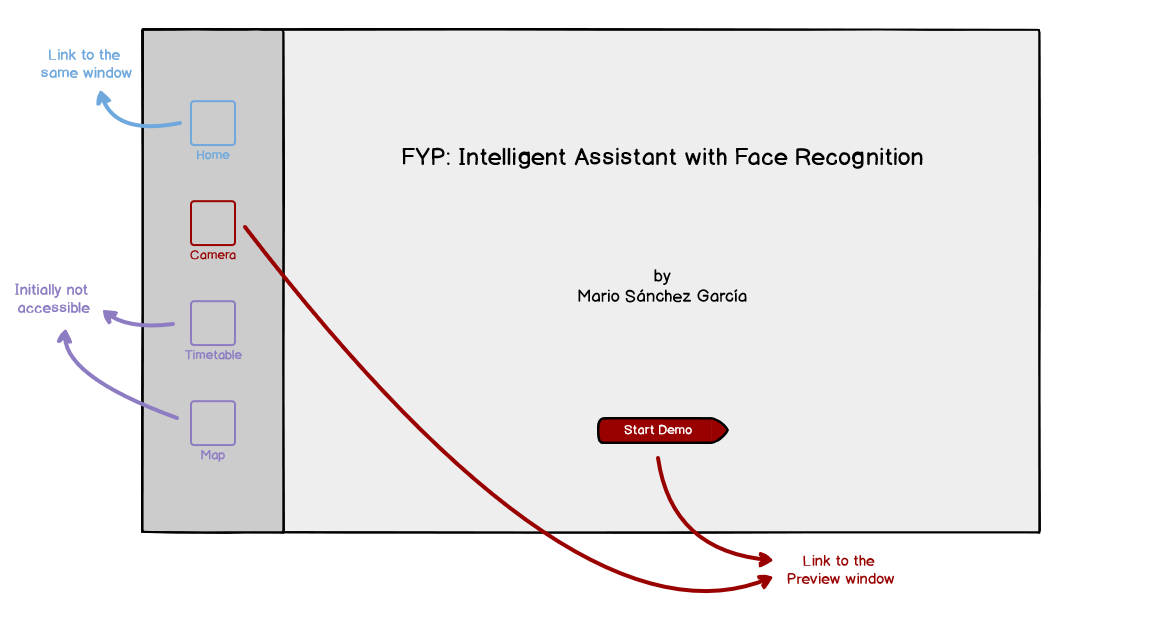
\includegraphics[width=15cm]{app_1_home_window.png}
		\caption{Home window of the application}
		\label{fig:home_window}
	\end{figure}

	\subsection{Preview window}
	\label{subsec:preview_window}

	This window (Figure \ref{fig:preview_window}) shows the a real time video stream of the camera, which will allow the users to have time to position themselves in front of the camera. In the lateral menu, the first icon links to the Home window (\ref{subsec:home_window}) and if it is clicked, the Home window will show up. The second links to this same window. The last two icons are disabled but still visible for the same reason of the previous window (the data needed to fill this windows has not been obtained yet).

	\begin{figure}[h!]
		\centering
		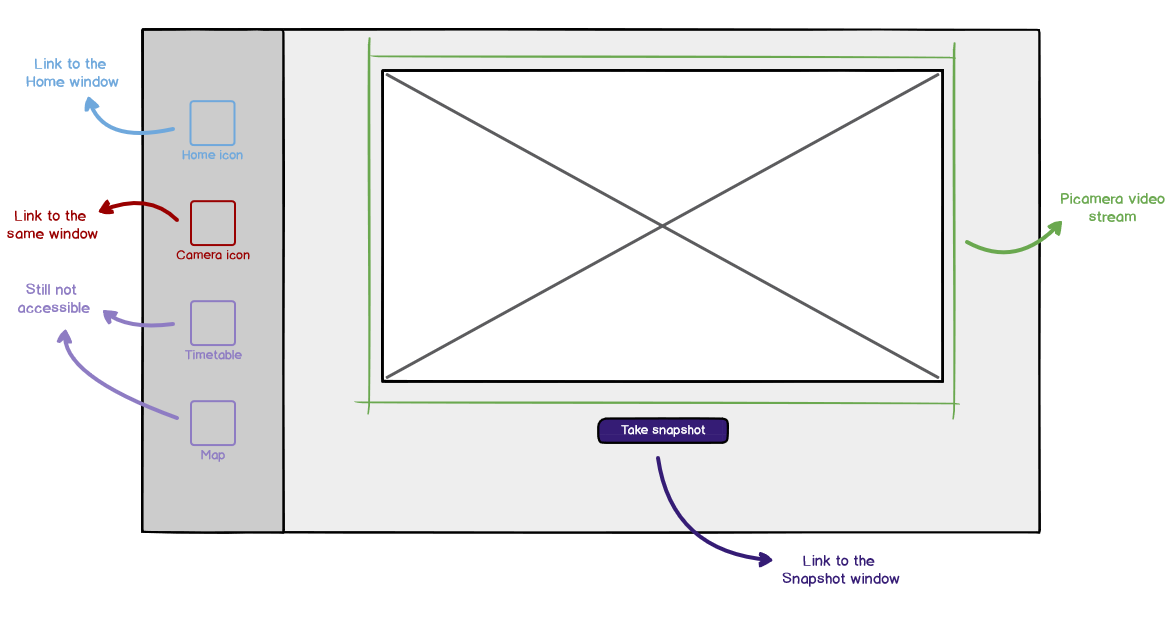
\includegraphics[width=15cm]{app_2_preview_window.png}
		\caption{Preview window of the application}
		\label{fig:preview_window}
	\end{figure}

	In the main panel of the right, the video stream of the \gls{picamera} is shown. The images of the stream have been flipped 180 degrees, as the camera is upside-down, and horizontally mirrored, so if the user moves to the right, the movement will be to the right in the preview as well. The button below the preview links to the Snapshot window (\ref{subsec:snapshot_window}) and will take the current video frame as the selected image in the moment it is clicked.

	\subsection{Snapshot window}
	\label{subsec:snapshot_window}
	This window (Figure \ref{fig:snap_window}) shows the image that was selected previously and that we will call \textit{\gls{snapshot}}. In the lateral menu, the first icon links to the Home window (\ref{subsec:home_window}) and if it is clicked, the Home window will show up. The second icon and the button "Take another snapshot" has the same action: show again the Preview window (\ref{subsec:preview_window}) and discard the current snapshot. The last two icons are disabled but still visible for the same reason of the Home window (the data needed to fill this windows has not been obtained yet).

	\begin{figure}[h!]
		\centering
		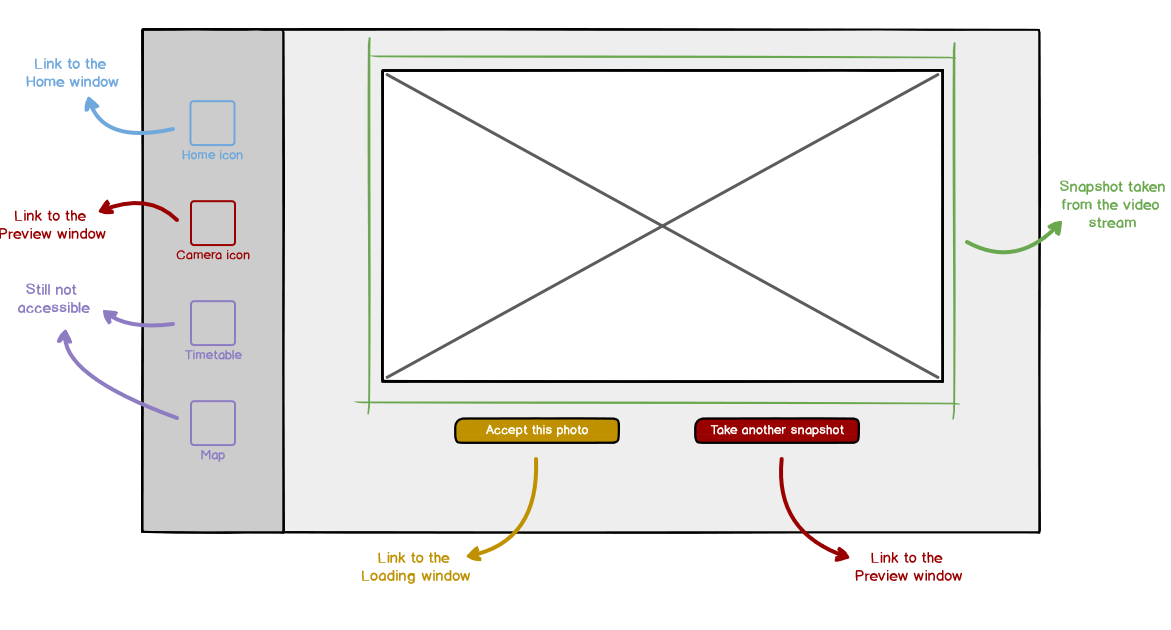
\includegraphics[width=15cm]{app_3_snap_window.png}
		\caption{Snapshot window of the application}
		\label{fig:snap_window}
	\end{figure}

	In the main panel of the right we can see the snapshot selected in the Preview window. The "Accept this photo" button links with the Loading window (\ref{subsec:loading_window}) and will send the snapshot to the server in order to identify the user as a student.

	\subsection{Loading window}
	\label{subsec:loading_window}
	This window (Figure \ref{fig:loading_window}) shows the progress in the communication with the server. All icons of the lateral menu will be disabled until the communication with the server is over. Depending of the call of the server that is being used at the moment, some icons of the menu will be different:

	\begin{itemize}
		\item Face recognition. The timetable icon will represent an user and it will be blinking each 0.5 seconds, being black in one phase and yellow in the other. 
		\item Get next class. The timetable icon will represent a calendar and it will be blinking each 0.5 seconds, being black in one phase and yellow in the other.
		\item Get map. The map icon will represent a map pin and it will be blinking each 0.5 seconds, being black in one phase and yellow in the other.
	\end{itemize}

	\begin{figure}[h!]
		\centering
		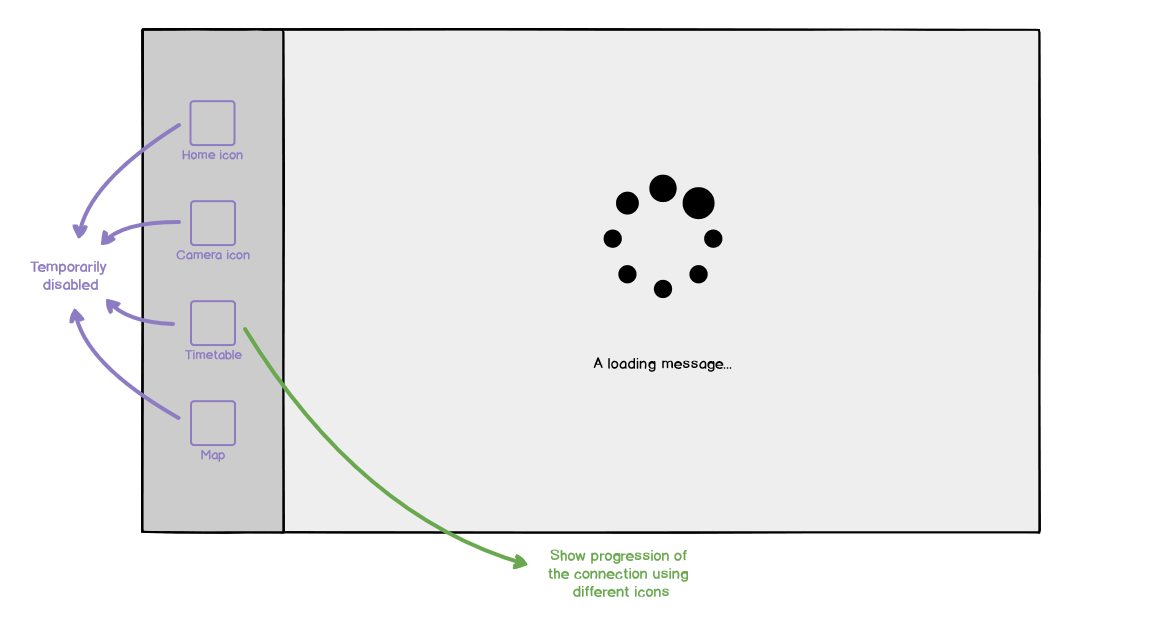
\includegraphics[width=15cm]{app_4_loading_window.png}
		\caption{Loading window of the application}
		\label{fig:loading_window}
	\end{figure}

	The snapshot from the previous window is sent to the server using a HTTP POST method to the route that it has for the face recognition service. The image is coded as UNICODE characters, so is can be wrapped using JSON. The server extracts the image from the request and decodes the JSON message to obtain again the original image. The server now applies the face detection proccess, where the faces detected are cropped out from the original image and saved in a new file. Now there are three possibilities depending of the output of this process (Figure \ref{fig:output_face_det}).

	\begin{figure}[h!]
		\centering
		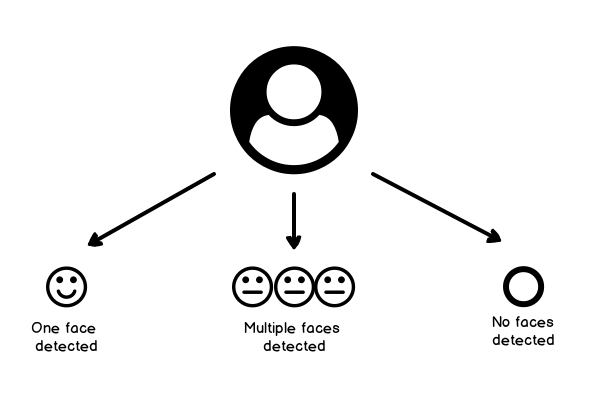
\includegraphics[width=9cm]{output_face_det.png}
		\caption{Possible outputs of the Face Detection process}
		\label{fig:output_face_det}
	\end{figure}

	The first possibility is that only one face is detected, which is the expected output of this process, being this face the one selected for the face recognition process. Another is that more than one face is detected, but in this case the first and leftmost face detected is the one selected for the face recognition process. The third and last possibility is that no faces are detected in the original image. Under these circumstances the server will send back a predefined default student instance along with a flag that will report the Raspberri Pi that no face could be detected. The Raspberry Pi will then show the Error window (\ref{subsec:error_window}) with a message informing the user about the situation.

	Following the expected output of the face detection process where only one face is detected, the face recognition process is applied to the new file with the cropped face. It will give back the student ID number of the recognised student with highest confidency percenteage (how sure is the \gls{cnn} of that the student in front of the camera is the recognised student) and the actual value of this confidency percenteage. 

	\begin{figure}[h!]
		\centering
		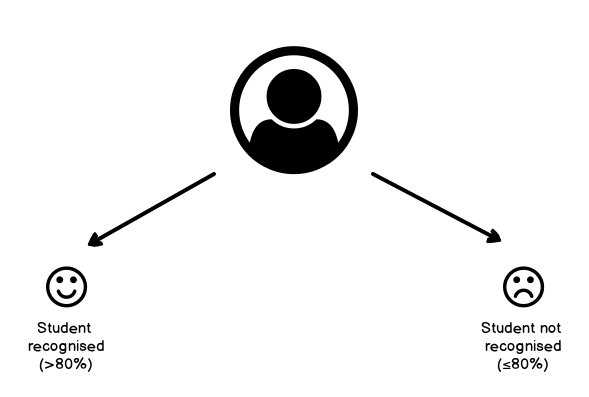
\includegraphics[width=9cm]{output_face_recog.png}
		\caption{Possible outputs of the Face Recognition process}
		\label{fig:output_face_recog}
	\end{figure}

	If the percenteage is less than 80\%, we will assume that the student is not recognised and therefore that the user is not a student. The system will follow a similar procedure to the no-face-detected case of before, but the flag sent will be different, informing that the student could not be detected. The Raspberry Pi will do the same as well, showing the Error window (\ref{subsec:error_window}) with a message to report the user about the situation. Otherwise, if the confidency percenteage is greater than 80\%, the server will take the name of the user from the database and send it along the ID number to the Raspberry Pi.

	Now that the Raspberry Pi knows the identity of the student, it will do another call to the server to get their next class of the day using the student's ID number. The server will use this ID to log into the timetable website of the University of Limerick (timetable.ul.ie). The website will give back as a response a static HTML page with a fixed pattern that contains the timetable. Analysing this pattern, the server will extract the timetable information from the fields of this HTML page and store it into a dictionary. Then, the current hour and weekday are taken into consideration to obtain the next class of the student.   

	\begin{figure}[h!]
		\centering
		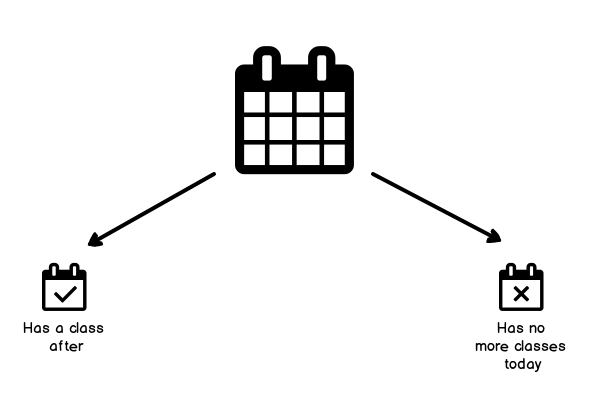
\includegraphics[width=9cm]{output_next_class.png}
		\caption{Possible outputs of the process of obtaining the next class}
		\label{fig:output_next_class}
	\end{figure}

	If the student has no more classes in the day, in the response a JSON is filled with a null value (\textit{None} in Python) and sent back. In this situation, the Raspberry Pi will show the No More Classes window (\ref{subsec:no_classes}) to inform the student about the situation. On the other hand, if the student actually has a next class, the previous referred JSON would be filled with the data of this class, which include: code of the module, name of the module, starting hour, ending hour, class type and location of the classroom.

	Finally, the Raspberry will use the class information to obtain the map from the server. The current location of the student and the location of the classroom, formatted as latitude and longitude coordinates, are sent to the server using the specific route for the map. The server will receive these locations and use them to construct first a link to obtain the path from one point to the other, and then another link to obtain the map image. This image is sent back to the Raspberry Pi, that uses all the gathered information to fill the Timetable (\ref{subsec:timetable_window}) and Map (\ref{subsec:map_window}) windows.

	Once the communication with the server is over and the windows have been updated, the application shows the Timetable window automatically.

	\subsection{Timetable window}
	\label{subsec:timetable_window}
	This window (Figure \ref{fig:timetable_window}) shows the a welcome message using the name of the recognised student and some information of the next class of this student, such as the code and name of the module, the location and the type of class. In the lateral menu now all icons are available. These icons are Home (\ref{subsec:home_window}), Camera (\ref{subsec:preview_window}), Timetable and Map. The last icon has the same function as the button that is placed in the main panel of the right, which is to link this window to the Map window (\ref{subsec:map_window}). 

	\begin{figure}[h!]
		\centering
		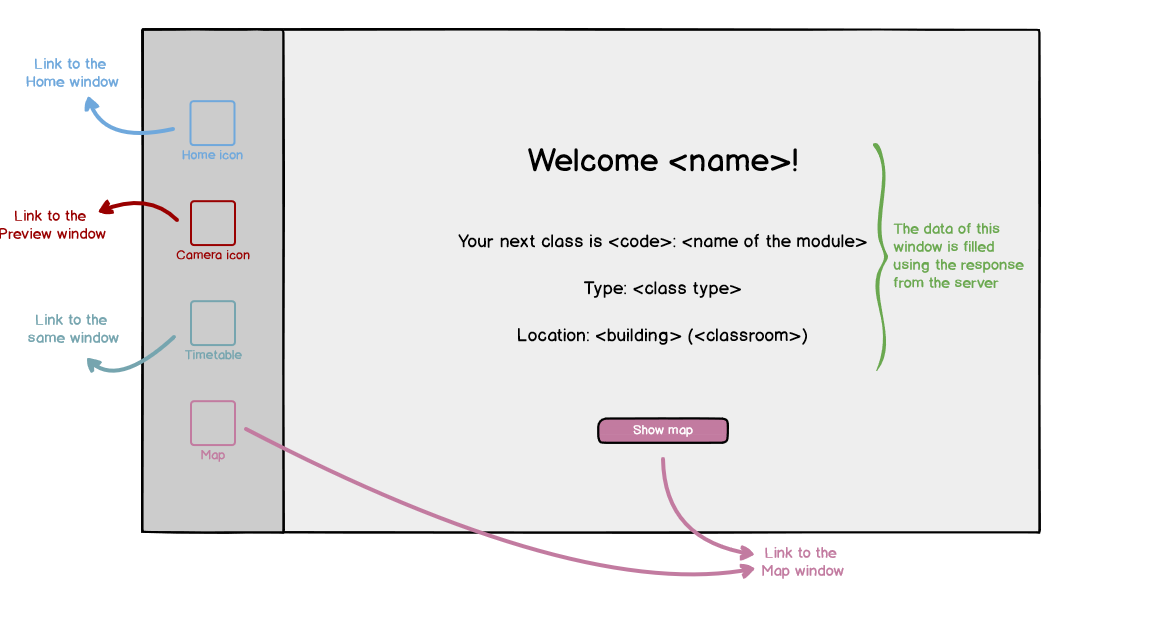
\includegraphics[width=15cm]{app_5_timetable_window.png}
		\caption{Timetable window of the application}
		\label{fig:timetable_window}
	\end{figure}

	\subsection{Map window}
	\label{subsec:map_window}
	This window (Figure \ref{fig:map_window}) shows the map to the next class of the student. In the lateral menu all icons are available. These buttons are These icons are Home (\ref{subsec:home_window}), Camera (\ref{subsec:preview_window}), Timetable (\ref{subsec:timetable_window}) and Map. In the top of the main panel of the right we can find the code and name of the module of the next class. Below it, the map image is displayed in a \gls{720p} resolution.

	\begin{figure}[h!]
		\centering
		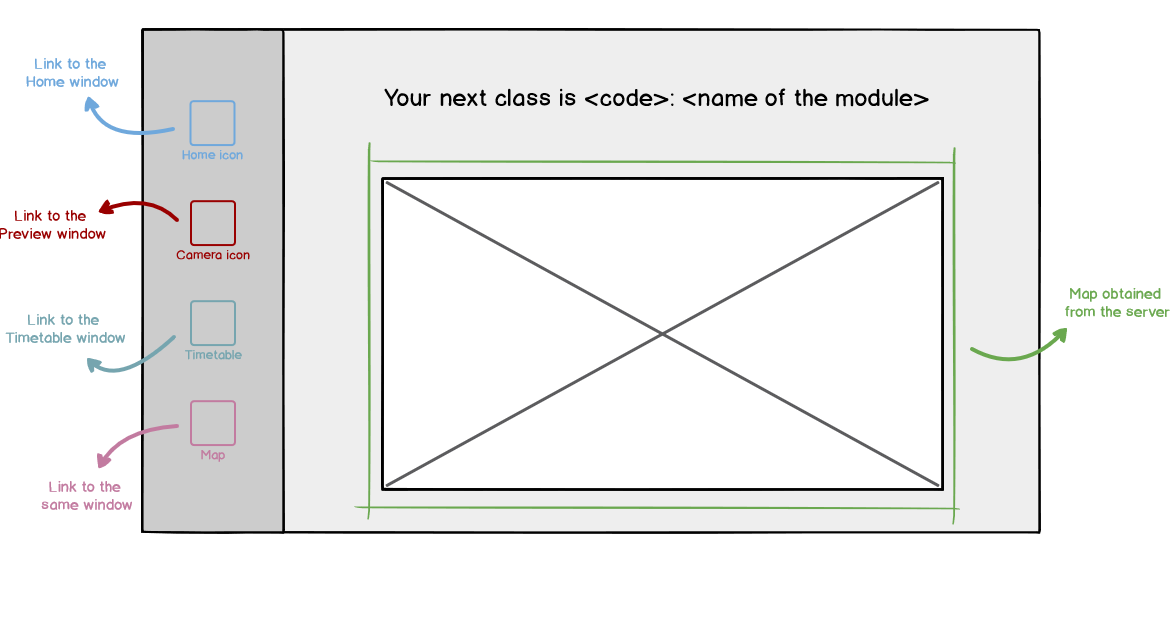
\includegraphics[width=15cm]{app_6_map_window.png}
		\caption{Map window of the application}
		\label{fig:map_window}
	\end{figure}

	\subsection{Error window}
	\label{subsec:error_window}
	This window (\ref{fig:error_window}) shows the user the kind of error that has occurred to the application. Only two possible errors are handled: \textit{no faces could be detected in the taken snapshot} or \textit{the user could not be identified as a student of the University of Limerick}. In both cases a message informing about the situation is displayed below a red cross icon in the main panel. 

	\begin{figure}[h!]
		\centering
		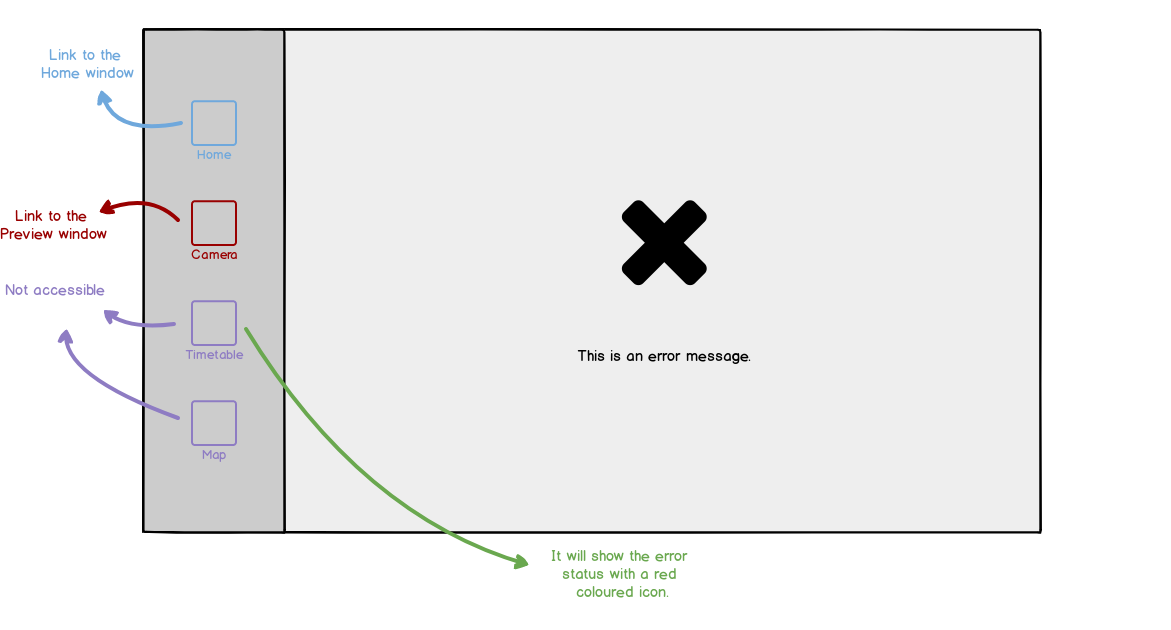
\includegraphics[width=15cm]{app_x_error_window}
		\caption{Error window of the application}
		\label{fig:error_window}
	\end{figure}	

	In the lateral menu we can find the Home and the Camera icons, that will link with the Home (\ref{subsec:home_window}) and Preview (\ref{subsec:preview_window}) windows, respectively. The third icon will represent a user using the red color instead of the usual Timetable icon and it will be disabled. When the user goes to another window from this point, this third icon will be still disabled but now showing the Timetable icon. The fourth and last icon will represent a Map pin, but as the map could not be obtained because of the error, it will be disabled.

	\subsection{No More Classes window}
	\label{subsec:no_classes}
	This window (\ref{fig:no_classes_window}) shows the user a welcome message using the name of the student and another message informing that the student has no more classes that day. In the lateral menu we can find the Home and the Camera icons, that will link with the Home (\ref{subsec:home_window}) and Preview (\ref{subsec:preview_window}) windows, respectively. The third will be the Timetable icon and in this case it will be not disabled.
	% When the user goes to another window from this point, this third icon will become disabled with the same icon.
	The fourth and last icon will represent a Map pin, but as the map could not be obtained because the user has no more classes, it will be disabled.

	\begin{figure}[h!]
		\centering
		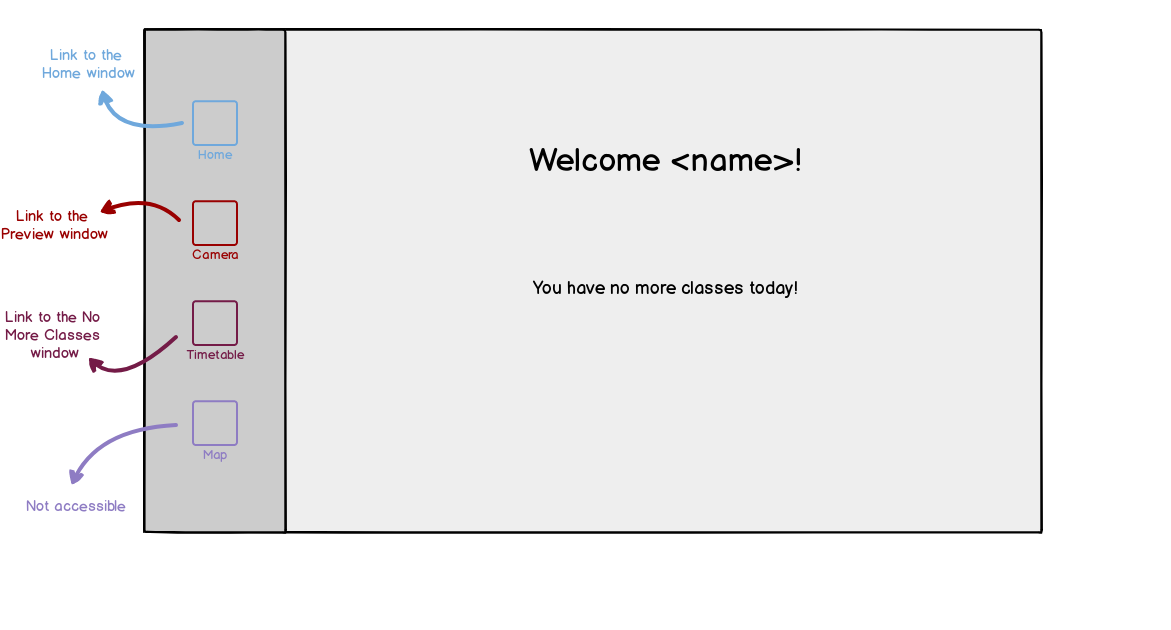
\includegraphics[width=15cm]{app_x_noclasses_window}
		\caption{No More Classes window of the application}
		\label{fig:no_classes_window}
	\end{figure}	



\section{Architecture and Technologies}
\label{sec:arch_n_tech}
\section{Front end}
\section{Back end}	
\section{Testing}
\section{Implementation issues}
\section{Summary of the implementation}
\section{Software Quality}





%\section{Related work}
%This section will include all the work that has been done for the project, but that is finally not included in the final version. For each related work, along with its explanation, we will also find the pros and cons of the solution and the reasons why it has not been included in the final version.
%	\subsection{Using Pi-Camera to stream}
%	As we explained in previous sections, the objective of the project is to capture (and after analyse) a photo of the face of a user, using the camera connected to the Raspberry Pi (Pi-Camera). Due to the limited scope of a Final Year Project, we added some constraints on how the photo should be, like that the face of the user must be centered in the photo or that they must look directly to the camera (in the Figure XX we can see an example of a photo). 
%
%	In order to provide to the users a way to place themselves correctly in front of the camera before the photo is taken, a preview is needed.	This preview must be shown in a screen, so assuming that the Raspberry Pi is not connected to it, we need a way to stream it in real-time to another computer (which will have a screen connected).
%
%	To start the development, we chose to use the code of an already written server that sends via HTTP a pre-recorded video (\cite{mjpeg_server_base_code}). In this project, the author aims to create "virtual cameras" using the format Motion JPEG (MJPEG), which is basically a sequence of JPEG images showed one after another. Until now, it fits perfectly for our Pi-camera, as it is able to capture in JPEG format.
%
%	However, the performance of this method is way worse than its competitor in the Raspberry Pi for video: h.264. Why choose MJPEG then? As we can see in \cite{mjpeg_format_info}, the MJPEG format "is natively supported by the QuickTime Player, the PlayStation console, and web browsers such as Safari, Google Chrome, Mozilla Firefox and Microsoft Edge". The four most used browsers support natively it, what takes away the work of create an application for the client side to show the stream. 
%
%	The GitHub project was designed to send a pre-recorded video, but we need a real-time video, so we changed the code to include the task of capturing the images. To do this task simultaneously with the image sending, we chose to use threads with a producer-consumer paradigm, synchronizing them using semaphores. The thread capturing the images acts as producer, and the one that computes the server is the consumer.    
%
%		\subsubsection{Pros and Cons}
%		Pros:
%		\begin{itemize}
%			\item Video format (MJPEG) is supported by the most used browsers natively.
%			\item This solution does not require the Raspberry Pi to be connected to the screen. 
%		\end{itemize}
%
%		Cons:
%		\begin{itemize}
%			\item The performance of the video format is poor, reaching a mean of 0.5fps after some testing.
%			\item The Raspberry Pi is included in the project to act as the user interface, so we don't need it away from the screen.
%			\item With only one core, the Raspberry Pi does not work well with threads.
%		\end{itemize}
%		
%		\subsubsection{Why is it not included in the final version?}
%		The poor performance of the stream makes difficult to place correctly the face in the camera, not only because of the mean 0.5 fps reached in the tests, but also for the delay that exits since the camera captures the photo until the browser shows it. 
